\section{Proving Undecidability by Reduction}

\begin{theorem}
    $A_{\mathsf{TF}}$ is not decidable.
\end{theorem}

\begin{proof}
    By contradiction.

    Suppose that $A_{\mathsf{TM}}$ is decidable. Then there exists some Turing machine that decides $A_{\mathsf{TM}}$. We will derive a contradiction by showing that if $A_{\mathsf{TM}}$ is decidable, then $\mathsf{DIAG}$ must also be decidable.

    To decide $\encoding{M} \in \mathsf{DIAG}$, we feed $\encoding{ M,\encoding{M} }$ into a Turing machine that decides $A_{\mathsf{TM}}$. 
\end{proof}

\begin{corollary}
    Let $\mathsf{D}$ be the class of decidable languages, and let $\mathsf{TR}$ is the class of Turing-recognizable.
    $$
    \mathsf{D} \subsetneq \mathsf{TR}
    $$
\end{corollary}

Let $\overline{A} = \{ w \in \Sigma^* \mid w \not\in A \} = \Sigma^* - A$.

Let $\coTR = \{ A \mid \overline{A} \in \mathsf{TR} \}$.

\begin{theorem}
    If $A \subseteq \Sigma^*$, then $A \in \mathsf{D} \iff A \in \TR\, \land\, \overline{A} \in \TR$.
\end{theorem}

\begin{proof}
    Suppose $A \in \TR \cap \coTR$. Let $M_1$ be a TM that recognizes $A$. Let $M_2$ be a TM that recognizes $\overline{A}$.

    Let $M$ be a multi-tape Turing machine that simulates $M_1$ and $M_2$ in parallel. On input $w$, since $w \in A$ or $w \not\in A$, either $M_1(w)$ accepts or $M_2(w)$ accepts. If $M_1$ accepts, then $M$ accepts. If $M_2$ accepts, then $M$ rejects.
\end{proof}

\section{Closure Properties}

\subsection{Union, Intersection, and Complement}

\begin{theorem}[Closure Under Union, Intersection, and Complement]
    If $A,B \in \D$, then $A \cup B \in \D$, $A \cap B \in \D$, and $\overline{A} \in \D$.
\end{theorem}

\begin{theorem}
    The class of languages $\TR$ is closed under union, intersection, but NOT under complement.
\end{theorem}

An intuitive explanation for why $\TR$ is not closed under complement, then this would imply that all languages in $\TR$ would also be decidable.

\begin{proof}
    Consider $A_{\TM} \in \TR$. If $\overline{A_{\TM}} \in \TR$, then $A_{\TM} \in \coTR$, which implies that $A_{\TM} \in \D$. A contradiction.  
\end{proof}

\begin{proof}
    Let $A,B \in \TR$. Then $A = L(M_1)$ and $B = L(M_2)$ for some TM $M_1$ and $M_2$.

    $A \cap B = L(M_{A\cap B})$ where $M_{AB}$ on input $w$ runs $M_1$ and $M_2$ in parallel on two tapes and accepts if and only if $M_1$ and $M_2$ both halts and accepts.

    $A \cup B = L(M_{A \cup B})$ where $M_{AB}$ on input $w$ runs $M_1$ and $M_2$ in parallel on two tapes and accepts if either $M_1$ or $M_2$ halts and accepts.
\end{proof}

\section{Computable Functions}

So far, we have been using TM to accept and reject inputs. However, we can also use a TM to compute a function. If a function can be computed (evaluated) using a Turing machine, we say the function is computable.

\begin{definition}[Computable Function]
    A function $f:\, \Sigma^* \to \Sigma^*$ is computable if there is some Turing machine $M$ on every input $w \in \Sigma^*$, $M$ halts with $f(w)$ on the tape.
\end{definition}

\begin{example}[Duplicate]
    Consider the function
    $f(w) = w \cdot w$ 
    that duplicates a string $w$.
\end{example}

Note that $f$ can take as input $\encoding(M)$ and output an encoding for some other Turing machine $\encoding{M'}$.

\begin{example}[Example of Uncomputable Function - Halting Problem]
    The function
    $$
    h(\encoding{\encoding{M},w}) = \begin{cases}
        1 & \text{if $M$ halts on input $w$} \\
        0 & \text{if $M$ does not halt on input $w$}
    \end{cases}
    $$
    solves the Halting problem and hence is not computable.
\end{example}

\begin{theorem}[Church-Turing Thesis]
    Any function that can be computed by an ``algorithm'', then the function is computable.
\end{theorem}

It can be shown by the diagonal argument that the set of all functions is uncountable, and hence not all functions are computable because the set of computable functions is countable.

\section{Mapping Reducible}

\begin{definition}[Mapping Reducible]
    A language $A$  is mapping reducible to $B$, denoted $A \leq_m B$ if there is a computable function $f:\; \Sigma^* \to \Sigma^*$ where for every $w$,
    $$
    w \in A \iff f(w) \in B
    $$
\end{definition}

\begin{figure}[htbp]
    \centering
    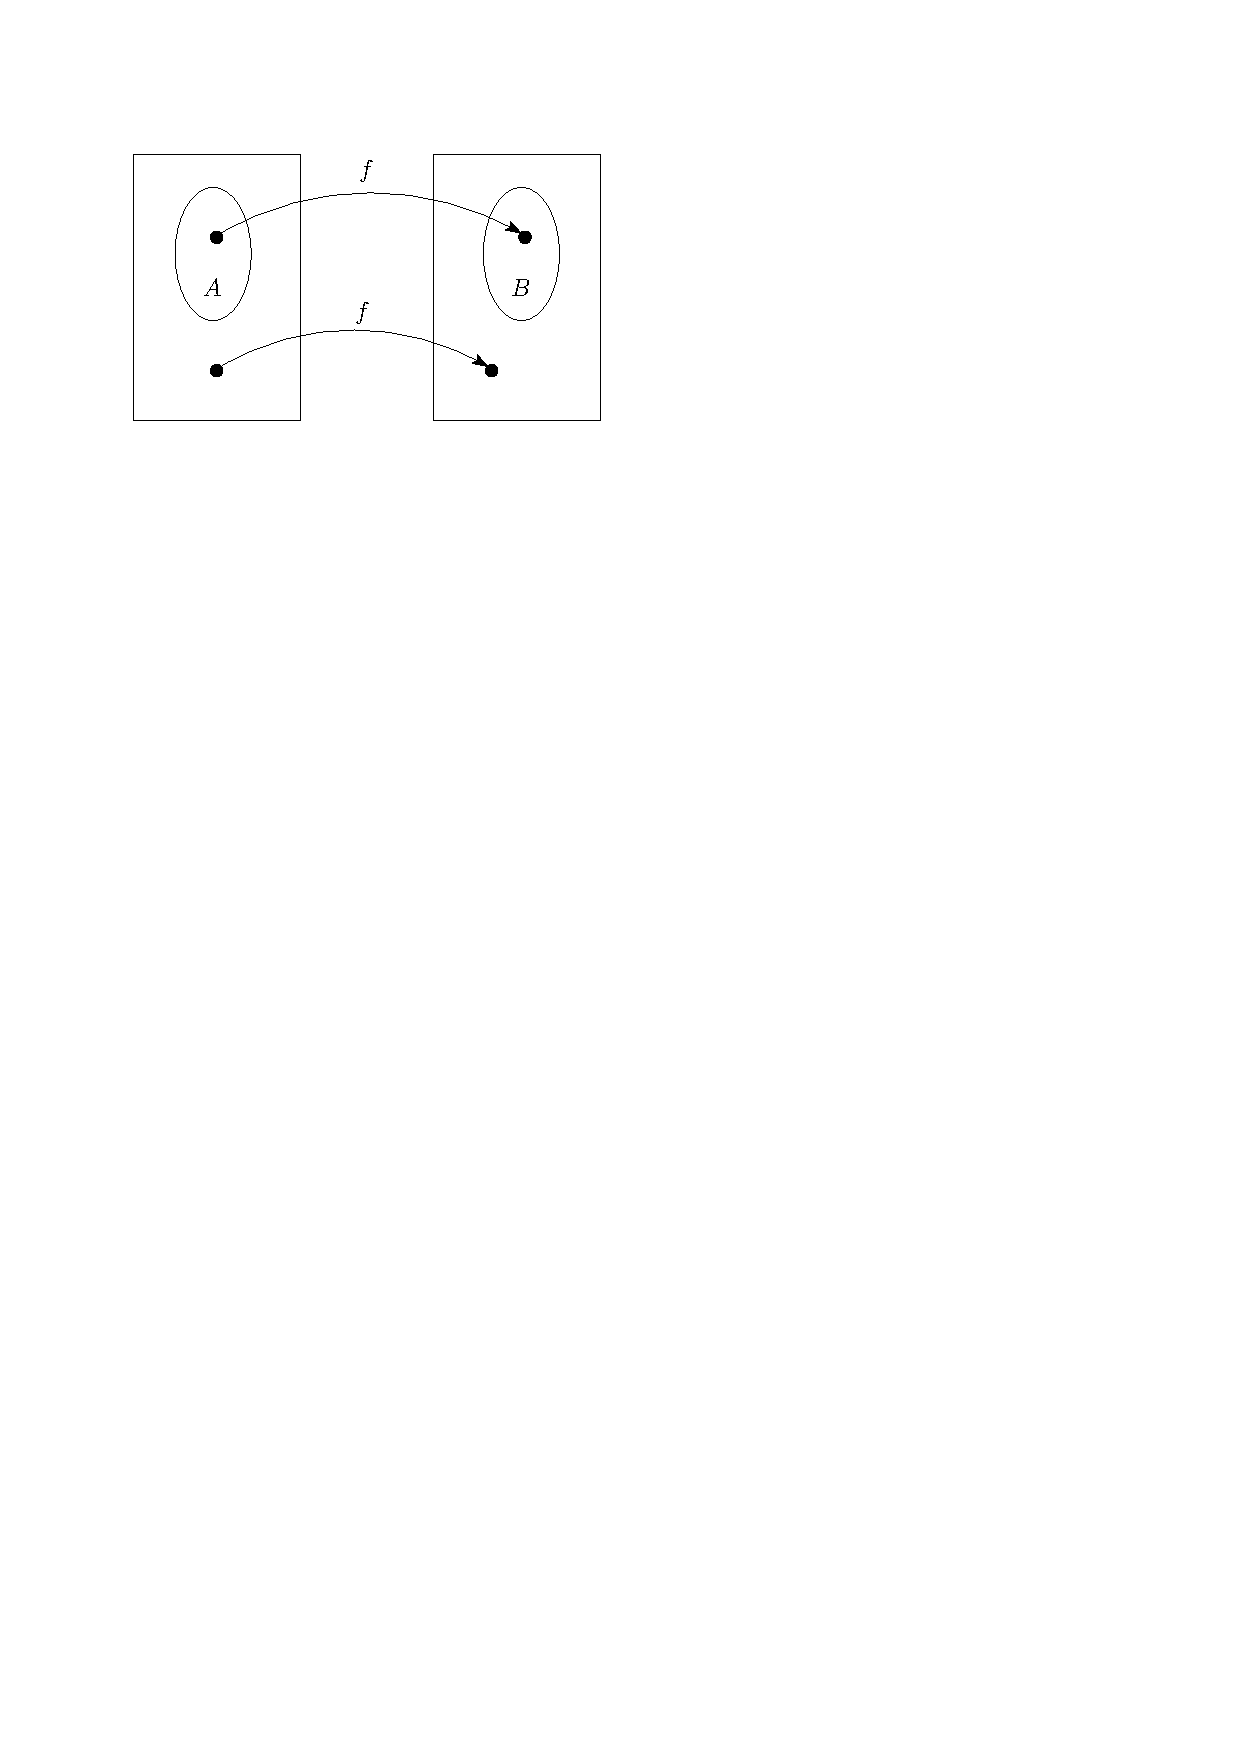
\includegraphics[width=0.4\linewidth]{mapping-reduction.pdf}
    \caption{Function $f$ reducing $A$ to $B$.}
    \label{fig:mapping-reduction}
\end{figure}

Observation: If $A \leq_m B$, then $\overline{A} \leq_m \overline{B}$. If $A \leq_m B$ and $B \leq_m C$, then $A \leq_m C$ (this follows from function composition).

\begin{remark}
    Later, we will see other types of reductions. For example, $\leq_p$ for polytime reduction.
\end{remark}

\begin{theorem}
    If $A \leq_m B$ and $B$ is decidable, then $A$ is decidable. If $B$ is Turing-recognizable, then $A$ is also Turing-recognizable.
\end{theorem}

\begin{proof}
    Let $M$ be a decider for $B$. Let $f$ be the computable mapping reduction from $A$ to $B$, and let $N$ be the Turing machine that computes this function.

    Then $A$ is decided by a Turing machine which on input $w$, runs $N$ to obtain $f(w)$ and then runs $M$ on $f(w)$.
\end{proof}

\begin{corollary}
    If $A \leq_m B$ and $A$ is not decidable, then $B$ is not decidable.
\end{corollary}

Application: Consider $\Diag = \{ \encoding{M} \mid \encoding{M} \not\in \lang(M) \}$. Then, $\Diag \leq_m \overline{A_{\TM}}$ via the reduction $f:\, \Sigma^* \to \Sigma^*$ defined as
$$
f(\encoding{M}) = \encoding{M,\encoding{M}}
$$
and if the input $w$ to $f$ is not an encoding of a TM, then
$$
f(w) = \encoding{M_{accept}, \epsilon}
$$

Since $\Diag$ is not decidable, $\overline{A_{\TM}}$ is not decidable.

\section{Applications of Reduction}

\subsection{Halting Problem}

Consider the language
$$
\Halt_{\TM} = \{ \encoding{M,w} \mid \text{$M$ halts on $w$} \}
$$

We have $\Halt_{\TM} \leq_m A_{\TM}$ and $A_{\TM} \leq_m \Halt_{\TM}$.

\begin{proof}

    \hfill
    
    ($\Halt_{\TM} \leq_m A_{\TM}$): If $x$ is any string of the form $\encoding{M,w}$, then $f(x) = \encoding{M',w}$ where $M'$ accepts if and only if $M$ halts on input $w$. $M'$ will simulate $M$ running on $w$ and accepts when $M$ halts. If $x$ is not of the correct form, $f(x) = \encoding{M_{loop},\epsilon}$.

    ($A_{\TM} \leq_m \Halt_{\TM}$): If $x$ is a string of the form $\encoding{M,w}$, then $f(x) = \encoding{M',w}$ where $M'$ simulates $M$ on $w$, and halts if and only if $M$ accepts. If $x$ is not of the correct form, then $f(x) = \encoding{M_{loop}, \epsilon}$.
\end{proof}

\begin{corollary}
    $\Halt_{\TM}$ is mapping equivalent (equivalent under mapping reduction) to $A_{\TM}$.
    $$
    \Halt_{\TM} \equiv_{m} A_{\TM}
    $$
\end{corollary}

Hence,
$$
\begin{aligned}
    \Halt_{\TM} &\in \TR \\
    &\not\in \coTR \\
    &\not\in \D
\end{aligned}
$$

\subsection{EQ}

Consider the language
$$
\EQ_{\TM} = \{ \encoding{M_1,M_2} \mid \text{$M_1$ and $M_2$ are Turing machines and $\lang(M_1) = \lang(M_2)$} \}
$$

We show that
$$
A_{\TM} \leq_{m} \EQ \qquad \text{and} \qquad A_{\TM} \leq_m \overline{\EQ}
$$

\begin{proof}
    Given $\encoding{M,w}$, if $M$ accepts $w$, we want to output $M_1,M_2$ such that $\lang(M_1) = \lang(M_2)$.

    Let $M_1$ be the TM which accepts all inputs. $\lang(M_1) = \Sigma^*$.
    
    Let $M_2$ be the TM which on any input, runs $M$ on $w$ and accepts if and only if $M$ accepts.

    So, $f(\encoding{M,w}) = \encoding{M_1,M_2}$.

    $$
    \lang(M_2) = \begin{cases}
        \Sigma^* & \text{if $M$ accepts $w$} \\
        \emptyset & \text{otherwise}
    \end{cases}
    $$

    Reduction from $A_{\TM}$ to $\overline{\EQ}$.
\end{proof}

Let $A$ be a set of TM descriptions $\{\encoding{M_1},\encoding{M_2},\ldots\}$. Show that if $A \in \TR$, then there is some set of TM descriptions $B \in \D$ such that the set of associated languages of $A$ and $B$ are the same. Formally,
$$
\{ \lang(M) \mid \encoding{M} \in A \} = \{ \lang(M) \mid \encoding{M} \in B \} 
$$
Let $E_B$ be an enumerator for $B$.
\begin{codebox}
    \li $\id{prev-length} = 0$
    \li \For $\encoding{M_1},\encoding{M_2},\ldots$ from $E_A$ \Do
        \li $M' = \proc{Pad}(\encoding{M_1},\, \id{prev-length} + 1)$
        \li $\id{prev-length} = |\encoding{M'}|$
        \li \textbf{print} $\encoding{M'}$
\end{codebox}
$\lang(E_B)$ is the decidable language that is the same as the language recognized by Turing machines in $A$.

Let $A \in \TR$ be a recognizable set of decider descriptions. Show that there is some decidable set $B$ such that $B$ is not the language of any TM in $A$.

Let $A = \{\encoding{D_1},\encoding{D_2},\ldots\}$. We want to show that there exists some $B$ such that $\forall i.\, B \not \in \lang(D_1)$. Let $\encoding{D_1},\encoding{D_2},\ldots$ be an enumeration of $A$. Also, let $w_1,w_2,\ldots$ be an enumeration of $\Sigma^*$ in standard string order.

Let $B = \{ w_i \mid w_i \not\in \lang(D_i) \}$. We first show that $B$ is decidable. We can construct a decider for $B$ as follows.
\begin{codebox}
    \Procname{$D_B(x)$}
    \li determine $i$ such that $w_i = x$
    \li run the enumerator for $A$ to get $\encoding{D_i}$ 
    \li simulate $D_i$ on $w_i = x$ 
    \li \If $D_i$ accepts \Then
        \li \textbf{reject}
    \li \Else
        \li \textbf{accept}
\end{codebox}

We then show that $B \not\in \lang(D_i)$ for some $\encoding{D_i} \in A$. If $w_i \in B$, then $w_i \not\in \lang(D_i)$, and $B \neq\lang(D_i)$. If $w_i \not\in B$, then $w_i \in \lang(D_i)$ and $B \neq \lang(D_i)$.

A language $A$ is recognizable if and only if there is a decider $V$ such that for all $x \in \Sigma^*$,
$$
x \in A \iff \exists y.\, \text{$V$ accepts $(x,y)$}
$$
Think $V$ as a verifier and $y$ as a ``certificate'' that $x \in A$.

$L$ is recognizable by TM $M$.
\begin{codebox}
    \Procname{$V(x,y)$}
    \li simulate $M$ on $x$ for $|y|$ steps
    \li \If $M$ accepts \Then
        \li \textbf{accept}
    \li \ElseIf $M$ rejects or has not completed \Then
        \li \textbf{reject}
    \End
\end{codebox}
If $x \in A$, then $M$ accepts within a finite number of steps $k$. Then, $V(x,\, y=1^k)$.

Now suppose that there exists a decider $V$ such that for all $x \in A$, there exists $y \in \Sigma^*$ such that $V$ accepts $(x,y)$.

We need to find a recognizer for $A$.

\begin{codebox}
    \Procname{$M(x)$}
    \li \For $y \in \Sigma^*$ \Do
        \li run $V(x,y)$ 
        \li \If $V$ accepts \Then
            \li \textbf{accept}
        \li \Else
            \li \textbf{continue}
\end{codebox}

If $x \in A$, there exists $y$ such that $V(x,y)$ accepts, then $y$ eventually show up in the standard string order of $\Sigma^*$ and when $y$ is run on $V$, $V$ accepts. Otherwise, $M$ loops.

\section{Rice's Theorem}

Using reduction, we can prove a really strong theorem about the decidability of certain languages, which can cover many of the languages that we have discussed so far.

\begin{theorem}[Rice's Theorem]
    Suppose $P$ is a language of Turing machine descriptions such that
    \begin{enumerate}
        \item $P$ is nontrivial: it contains some but not all Turing machine descriptions;
        \item $P$ is a \textit{\textbf{property of the Turing machine's languages}} (instead of a property of the Turing machine itself): whenever $\lang(M_1) = \lang(M_2)$, then $\encoding{M_1} \in P \iff \encoding{M_2} \in P$.  
    \end{enumerate}
    Then, $P$ is decidable.
\end{theorem}

Here are some example languages that are covered by Rice's theorem.
\begin{example}
    \hfill
    \begin{itemize}
        \item $\mathrm{EMPTY}_{\TM} = \{ \encoding{M} \mid \lang(M) = \emptyset \}$
        \item $\mathrm{FINITE}_{\TM} = \{ \encoding{M} \mid \text{$\lang(M)$ is finite} \}$
        \item $\mathrm{DECIDABLE}_{\TM} = \{ \encoding{M} \mid \text{$\lang(M)$ is decidable} \}$
    \end{itemize}
    Rice's theorem claims that all of these languages are undecidable.

    Note that Rice's theorem does not apply to $\{ \encoding{M} \mid \text{$M$ is a decider} \}$ because the property being satisfied by the TM descriptions in this language is a property of the Turing machine itself, not its language. Criterion 2 of Rice's theorem is not satisfied.
\end{example}

Now, let's prove Rice's theorem using reduction.

\begin{proof}
    Let $T_0$ be the TM which always rejects. Without loss of generality, suppose that $\encoding{T_0} \not\in P$. Otherwise, we can consider $\overline{P}$ which also satisfies the criteria for Rice's theorem.
    
    Since $P$ is nontrivial, there exists TM $T_1$ such that $\encoding{T_1} \in P$. We will show that $\ATM \leq_m P$. In this end, we map $\encoding{M,w}$ to $M_w$ where
    $$
    \begin{aligned}
        M_w = ``
        &\text{on input $x$} \\
        &\text{1. Simulate $M$ on $w$} \\
        &\text{2. If $M$ rejects $w$, reject} \\
        &\begin{aligned}
            \text{3. } &\text{If $M$ accepts $w$, then run $T_1$ on $x$} \\
            &\text{$M_w$ accepts/rejects/loops according to what $T_1$ does on input $x$}"
        \end{aligned}
    \end{aligned}
    $$
    $\lang(M_w)$ is either $\emptyset = \lang(T_0)$ or the langauge of $T_1$, $\lang(T_1)$, depending on whether $w$ is accepted by $M$.

    \textit{Claim}. $\encoding{M,w} \in \ATM \iff \encoding{M_w} \in P$.

    If $M$ accepts $w$, then $\lang(M_w) = \lang(T_1)$, so $M_w \in P$. \\
    If $M$ rejects $w$, then $\lang(M_w) = \emptyset = \lang(T_0)$, so $\encoding{M_w} \not\in P$. \\
    If $M$ loops on $w$, $M_w$ loops on all inputs so $\lang(M_w) = \emptyset = \lang(T_0)$.
\end{proof}